\documentclass[]{article}
\usepackage{lmodern}
\usepackage{amssymb,amsmath}
\usepackage{ifxetex,ifluatex}
\usepackage{fixltx2e} % provides \textsubscript
\ifnum 0\ifxetex 1\fi\ifluatex 1\fi=0 % if pdftex
  \usepackage[T1]{fontenc}
  \usepackage[utf8]{inputenc}
\else % if luatex or xelatex
  \ifxetex
    \usepackage{mathspec}
  \else
    \usepackage{fontspec}
  \fi
  \defaultfontfeatures{Ligatures=TeX,Scale=MatchLowercase}
\fi
% use upquote if available, for straight quotes in verbatim environments
\IfFileExists{upquote.sty}{\usepackage{upquote}}{}
% use microtype if available
\IfFileExists{microtype.sty}{%
\usepackage{microtype}
\UseMicrotypeSet[protrusion]{basicmath} % disable protrusion for tt fonts
}{}
\usepackage[margin=1in]{geometry}
\usepackage{hyperref}
\hypersetup{unicode=true,
            pdftitle={Chicago Crime Data Analysis},
            pdfauthor={Student ID:/ 201081646},
            pdfborder={0 0 0},
            breaklinks=true}
\urlstyle{same}  % don't use monospace font for urls
\usepackage{color}
\usepackage{fancyvrb}
\newcommand{\VerbBar}{|}
\newcommand{\VERB}{\Verb[commandchars=\\\{\}]}
\DefineVerbatimEnvironment{Highlighting}{Verbatim}{commandchars=\\\{\}}
% Add ',fontsize=\small' for more characters per line
\usepackage{framed}
\definecolor{shadecolor}{RGB}{248,248,248}
\newenvironment{Shaded}{\begin{snugshade}}{\end{snugshade}}
\newcommand{\KeywordTok}[1]{\textcolor[rgb]{0.13,0.29,0.53}{\textbf{{#1}}}}
\newcommand{\DataTypeTok}[1]{\textcolor[rgb]{0.13,0.29,0.53}{{#1}}}
\newcommand{\DecValTok}[1]{\textcolor[rgb]{0.00,0.00,0.81}{{#1}}}
\newcommand{\BaseNTok}[1]{\textcolor[rgb]{0.00,0.00,0.81}{{#1}}}
\newcommand{\FloatTok}[1]{\textcolor[rgb]{0.00,0.00,0.81}{{#1}}}
\newcommand{\ConstantTok}[1]{\textcolor[rgb]{0.00,0.00,0.00}{{#1}}}
\newcommand{\CharTok}[1]{\textcolor[rgb]{0.31,0.60,0.02}{{#1}}}
\newcommand{\SpecialCharTok}[1]{\textcolor[rgb]{0.00,0.00,0.00}{{#1}}}
\newcommand{\StringTok}[1]{\textcolor[rgb]{0.31,0.60,0.02}{{#1}}}
\newcommand{\VerbatimStringTok}[1]{\textcolor[rgb]{0.31,0.60,0.02}{{#1}}}
\newcommand{\SpecialStringTok}[1]{\textcolor[rgb]{0.31,0.60,0.02}{{#1}}}
\newcommand{\ImportTok}[1]{{#1}}
\newcommand{\CommentTok}[1]{\textcolor[rgb]{0.56,0.35,0.01}{\textit{{#1}}}}
\newcommand{\DocumentationTok}[1]{\textcolor[rgb]{0.56,0.35,0.01}{\textbf{\textit{{#1}}}}}
\newcommand{\AnnotationTok}[1]{\textcolor[rgb]{0.56,0.35,0.01}{\textbf{\textit{{#1}}}}}
\newcommand{\CommentVarTok}[1]{\textcolor[rgb]{0.56,0.35,0.01}{\textbf{\textit{{#1}}}}}
\newcommand{\OtherTok}[1]{\textcolor[rgb]{0.56,0.35,0.01}{{#1}}}
\newcommand{\FunctionTok}[1]{\textcolor[rgb]{0.00,0.00,0.00}{{#1}}}
\newcommand{\VariableTok}[1]{\textcolor[rgb]{0.00,0.00,0.00}{{#1}}}
\newcommand{\ControlFlowTok}[1]{\textcolor[rgb]{0.13,0.29,0.53}{\textbf{{#1}}}}
\newcommand{\OperatorTok}[1]{\textcolor[rgb]{0.81,0.36,0.00}{\textbf{{#1}}}}
\newcommand{\BuiltInTok}[1]{{#1}}
\newcommand{\ExtensionTok}[1]{{#1}}
\newcommand{\PreprocessorTok}[1]{\textcolor[rgb]{0.56,0.35,0.01}{\textit{{#1}}}}
\newcommand{\AttributeTok}[1]{\textcolor[rgb]{0.77,0.63,0.00}{{#1}}}
\newcommand{\RegionMarkerTok}[1]{{#1}}
\newcommand{\InformationTok}[1]{\textcolor[rgb]{0.56,0.35,0.01}{\textbf{\textit{{#1}}}}}
\newcommand{\WarningTok}[1]{\textcolor[rgb]{0.56,0.35,0.01}{\textbf{\textit{{#1}}}}}
\newcommand{\AlertTok}[1]{\textcolor[rgb]{0.94,0.16,0.16}{{#1}}}
\newcommand{\ErrorTok}[1]{\textcolor[rgb]{0.64,0.00,0.00}{\textbf{{#1}}}}
\newcommand{\NormalTok}[1]{{#1}}
\usepackage{graphicx,grffile}
\makeatletter
\def\maxwidth{\ifdim\Gin@nat@width>\linewidth\linewidth\else\Gin@nat@width\fi}
\def\maxheight{\ifdim\Gin@nat@height>\textheight\textheight\else\Gin@nat@height\fi}
\makeatother
% Scale images if necessary, so that they will not overflow the page
% margins by default, and it is still possible to overwrite the defaults
% using explicit options in \includegraphics[width, height, ...]{}
\setkeys{Gin}{width=\maxwidth,height=\maxheight,keepaspectratio}
\IfFileExists{parskip.sty}{%
\usepackage{parskip}
}{% else
\setlength{\parindent}{0pt}
\setlength{\parskip}{6pt plus 2pt minus 1pt}
}
\setlength{\emergencystretch}{3em}  % prevent overfull lines
\providecommand{\tightlist}{%
  \setlength{\itemsep}{0pt}\setlength{\parskip}{0pt}}
\setcounter{secnumdepth}{5}
% Redefines (sub)paragraphs to behave more like sections
\ifx\paragraph\undefined\else
\let\oldparagraph\paragraph
\renewcommand{\paragraph}[1]{\oldparagraph{#1}\mbox{}}
\fi
\ifx\subparagraph\undefined\else
\let\oldsubparagraph\subparagraph
\renewcommand{\subparagraph}[1]{\oldsubparagraph{#1}\mbox{}}
\fi

%%% Use protect on footnotes to avoid problems with footnotes in titles
\let\rmarkdownfootnote\footnote%
\def\footnote{\protect\rmarkdownfootnote}

%%% Change title format to be more compact
\usepackage{titling}

% Create subtitle command for use in maketitle
\newcommand{\subtitle}[1]{
  \posttitle{
    \begin{center}\large#1\end{center}
    }
}

\setlength{\droptitle}{-2em}
  \title{Chicago Crime Data Analysis}
  \pretitle{\vspace{\droptitle}\centering\huge}
  \posttitle{\par}
  \author{Student ID:/ 201081646}
  \preauthor{\centering\large\emph}
  \postauthor{\par}
  \predate{\centering\large\emph}
  \postdate{\par}
  \date{November 3, 2018}


\begin{document}
\maketitle

\section{Introduction}\label{introduction}

This is the first assessment for the \textbf{MATH5741M Statistical
Theory and Methods} module. Its objective is to summarise statistically
a crime dataset sample from the city of Chicago and answer the following
research questions:

\begin{itemize}
\item
  What time of day do most types of crime occur?
\item
  In which locations are specific types of crime more likely to happen?
\item
  Which districts are potentially more dangerous per type of crime?
\end{itemize}

\section{Data and methods}\label{data-and-methods}

The dataset analysed is a sample of the
\href{https://data.cityofchicago.org/Public-Safety/Crimes-2001-to-present/ijzp-q8t2}{original
data of crimes extracted from the Chicago Police Department} that
occurred in the city of Chicago from 2001 to present.

For the analysis, first, we prepare the data creating, transforming and
simplifying variables, as well as cleaning the dataset keeping the
variables we are interested in. Secondly, we make a general univariable
analysis of the data set, and then, with a multianalysys based on
heatmaps we answer our questions. Finally, we sumarise the findings.

The report describes not only the statistical process followed but also
incorporates the most important R code used to carry it out.
Unfortunately, space constraints did not allow to include all the code
use, however it is available in
\url{https://github.com/eugenividal/Chicago-Crime-Data-Analysis}.

\section{Results}\label{results}

\subsection{Data preparation}\label{data-preparation}

First, we load the data into the \texttt{R} environment.

\begin{Shaded}
\begin{Highlighting}[]
\CommentTok{# read csv in R}
\NormalTok{dd=}\KeywordTok{read.csv}\NormalTok{(}\StringTok{"http://www1.maths.leeds.ac.uk/~charles/math5741/crime.csv"}\NormalTok{,}\DataTypeTok{header=}\NormalTok{T)}
\end{Highlighting}
\end{Shaded}

Second, we create new variables (\texttt{count}, \texttt{hour}) based on
the existing ones, and give them the right format for later explotation.

Third, we simplify the variables \texttt{Primary.Type} and
\texttt{Location.Description} grouping their categories and call them
\texttt{Type\_grouped} and \texttt{Location\_grouped} respectivelly.

Next, we keep only those variables which will help us to answer our
questions. So, we drop all the variable we do not need.

\begin{Shaded}
\begin{Highlighting}[]
\CommentTok{# Drop all variables we are not interested in}
\NormalTok{dd <-}\StringTok{ }\NormalTok{dd[, -}\KeywordTok{c}\NormalTok{(}\DecValTok{1}\NormalTok{:}\DecValTok{8}\NormalTok{, }\DecValTok{10}\NormalTok{:}\DecValTok{11}\NormalTok{, }\DecValTok{13}\NormalTok{:}\DecValTok{18}\NormalTok{)]}
\end{Highlighting}
\end{Shaded}

Then, we clean the dataset of missing values.

\begin{Shaded}
\begin{Highlighting}[]
\CommentTok{# Remove NAs}
\NormalTok{dd <-}\StringTok{ }\NormalTok{dd[}\KeywordTok{complete.cases}\NormalTok{(dd),]}
\end{Highlighting}
\end{Shaded}

Finally, the data is ready for the explotation.

\begin{Shaded}
\begin{Highlighting}[]
\KeywordTok{head}\NormalTok{(dd)}
\end{Highlighting}
\end{Shaded}

\begin{verbatim}
##   Arrest District count hour   Month_Yr Type_grouped Location_grouped
## 1   true       19     1   00 2013-07-01       Batery           Street
## 2   true       19     1   01 2013-07-01       Others           Street
## 3  false        2     1   21 2013-07-01      Assault        Apartment
## 4   true        9     1   02 2013-07-01    Narcotics           Street
## 5  false        3     1   17 2013-07-01        Theft           Street
## 6   true        9     1   01 2013-07-01       Batery        Apartment
\end{verbatim}

\subsection{Data exploration}\label{data-exploration}

\subsubsection{General analysis}\label{general-analysis}

\paragraph{Crime evolution}\label{crime-evolution}

The number of crimes in Chicago has decrease dramatically per year from
2001 to present.

\begin{figure}[htbp]
\centering
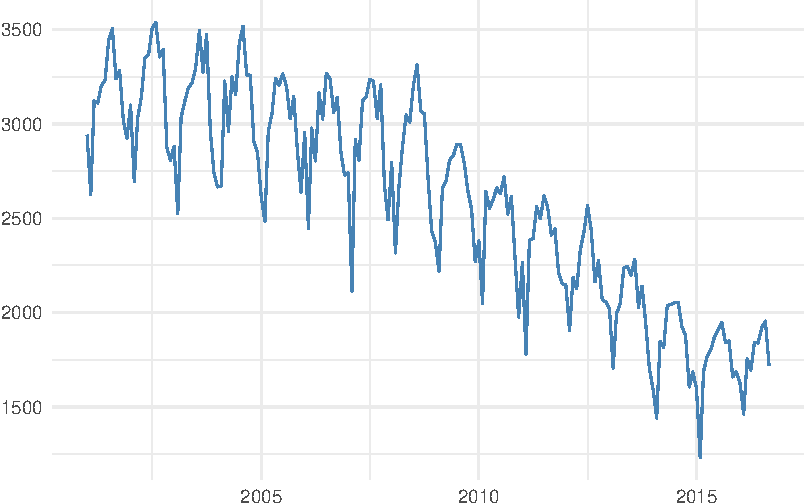
\includegraphics{Assessment_1v7_files/figure-latex/fig-1.pdf}
\caption{Crimes evolution}
\end{figure}

Except for the deceptive practice, all the crimes have decresead in more
or less grade.

\begin{figure}[htbp]
\centering
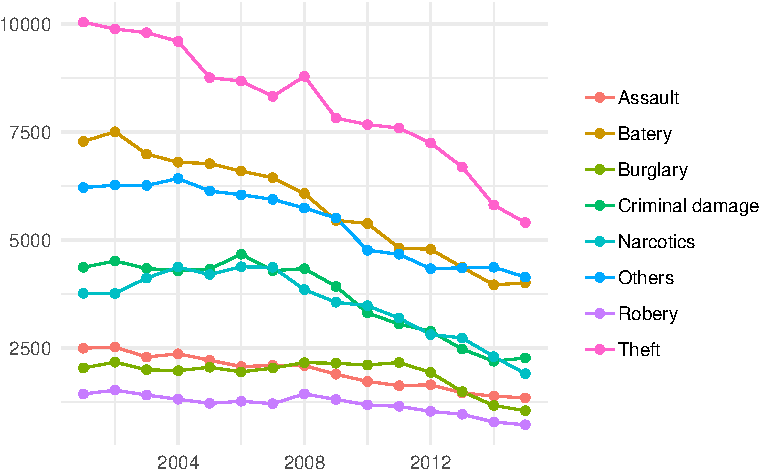
\includegraphics{Assessment_1v7_files/figure-latex/fig2-1.pdf}
\caption{Evolution per type of crime}
\end{figure}

\paragraph{Crime per hour}\label{crime-per-hour}

The crimes are concentrated in hours

\begin{figure}[htbp]
\centering
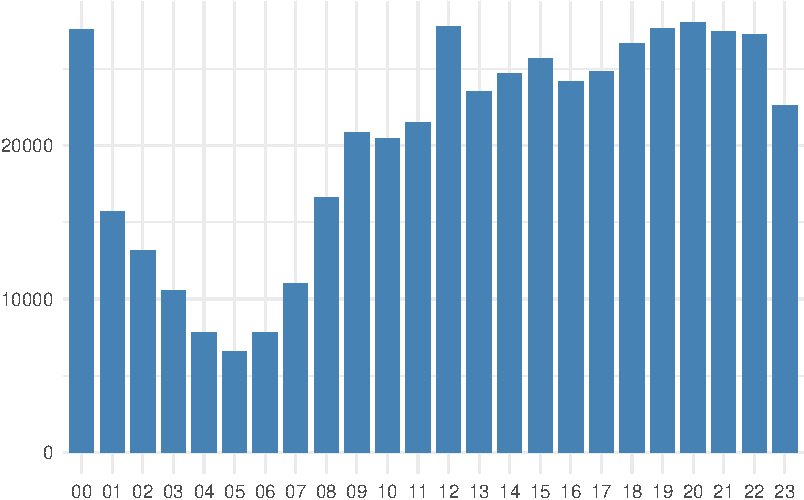
\includegraphics{Assessment_1v7_files/figure-latex/fig3-1.pdf}
\caption{Crimes per hour}
\end{figure}

\paragraph{Type of crimes}\label{type-of-crimes}

Per type of crime Theft is in difference the biggest number. Change the
scientifyc number.

\begin{figure}[htbp]
\centering
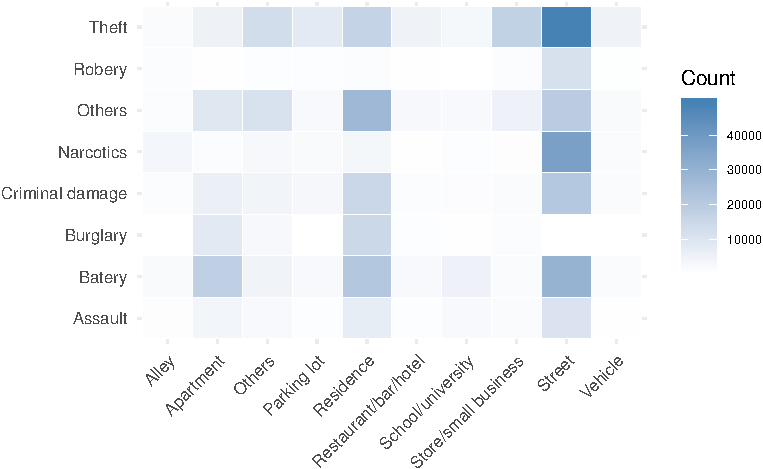
\includegraphics{Assessment_1v7_files/figure-latex/fig6-1.pdf}
\caption{Crimes per type}
\end{figure}

\paragraph{Location of crimes}\label{location-of-crimes}

These crimes are concentrated in Streets, give percentage.

\begin{figure}[htbp]
\centering
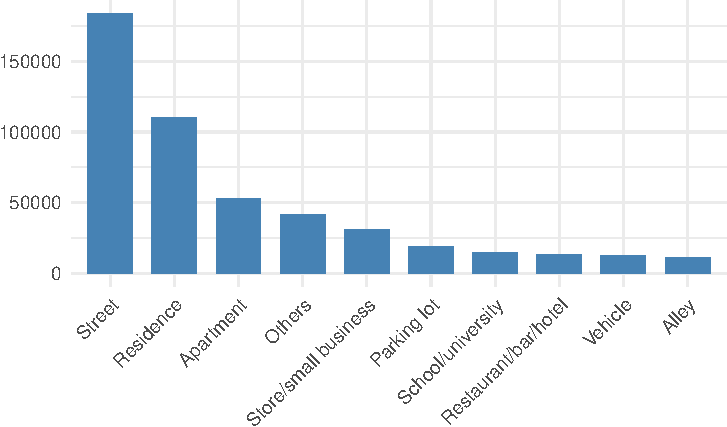
\includegraphics{Assessment_1v7_files/figure-latex/fig7-1.pdf}
\caption{Crimes per location}
\end{figure}

\paragraph{Crime per districts}\label{crime-per-districts}

Per districts the most dangerous are 8.

\subsubsection{Answers to our questions}\label{answers-to-our-questions}

The multiple analysis focuses on type of crime crossed with hour,
location and district.

\paragraph{What time of day do most types of crime
occur?}\label{what-time-of-day-do-most-types-of-crime-occur}

Are some types of crimes more likely to happen in specific time of the
day?

The most dangerous hours per Thefth are 00 and 12.

\begin{figure}[htbp]
\centering
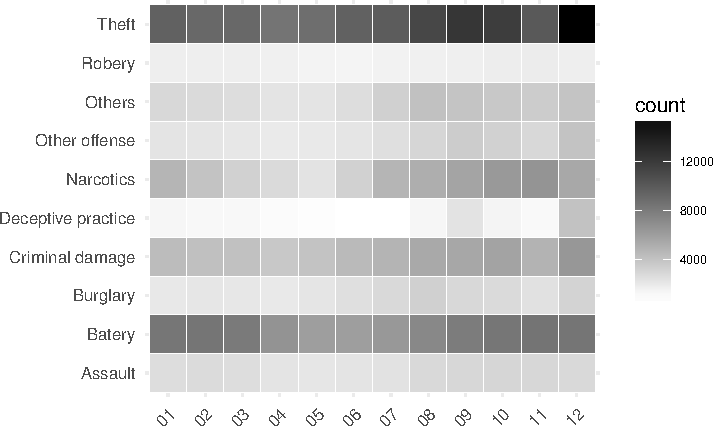
\includegraphics{Assessment_1v7_files/figure-latex/fig9-1.pdf}
\caption{Type of crime vs hour}
\end{figure}

\paragraph{In which locations are specific types of crime more likely to
happen?}\label{in-which-locations-are-specific-types-of-crime-more-likely-to-happen}

Are some types of crimes more likely to happen in specific locations?

Street is particularly important for Theft.

\begin{figure}[htbp]
\centering
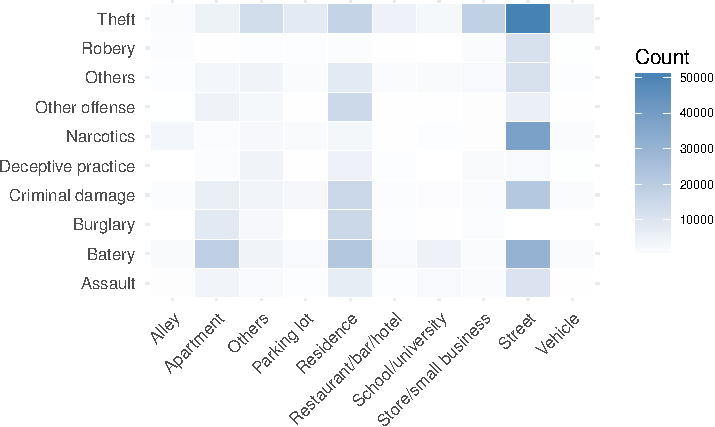
\includegraphics{Assessment_1v7_files/figure-latex/fig11-1.pdf}
\caption{Type of crime vs location}
\end{figure}

\paragraph{Which districts are potentially more dangerous per type of
crime?}\label{which-districts-are-potentially-more-dangerous-per-type-of-crime}

Are some types of crimes more likely to happen in specific distrits?

Narcotics in district 11 is crealy a problem.

\begin{figure}[htbp]
\centering
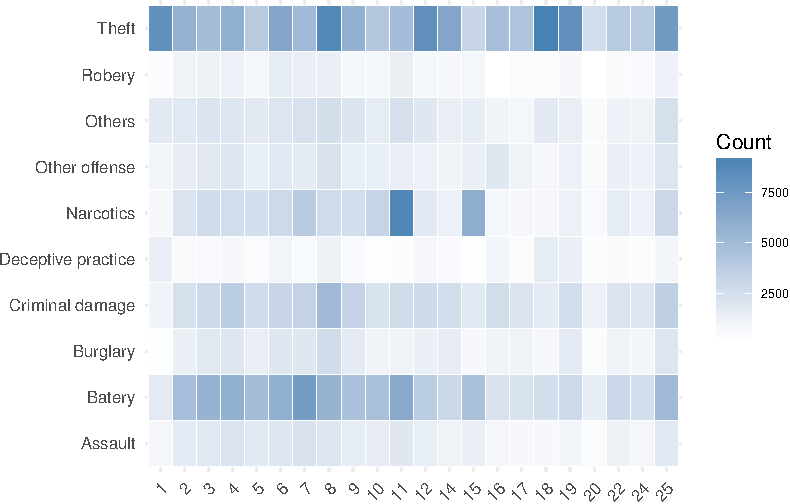
\includegraphics{Assessment_1v7_files/figure-latex/fig10-1.pdf}
\caption{Type of crime vs district}
\end{figure}

\section{Conclusions}\label{conclusions}


\end{document}
